% Bagian Topologi
\section*{Topologi} % Jika ada lampiran

Pada modul ini, terdapat tiga topologi yang akan dibuat, yaitu:

\begin{itemize}
    \item Topologi 1: Point-to-Point
    \begin{figure}[H]
        \centering
        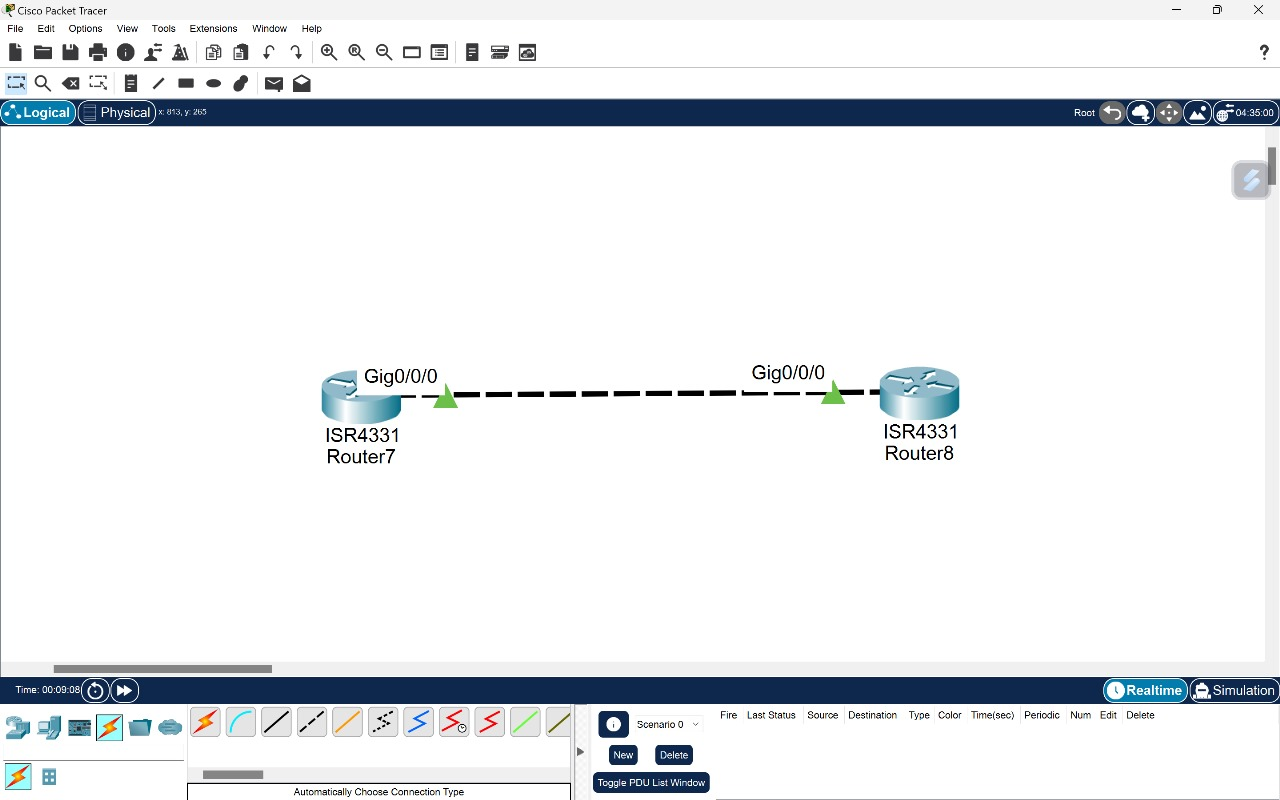
\includegraphics[width=0.6\textwidth]{img/point-point.jpeg}
        \caption{Topologi 1: Point-to-Point}
        \label{fig:topo1}
    \end{figure}
    \item Topologi 2: Point-to-Multipoint
    \begin{figure}[H]
        \centering
        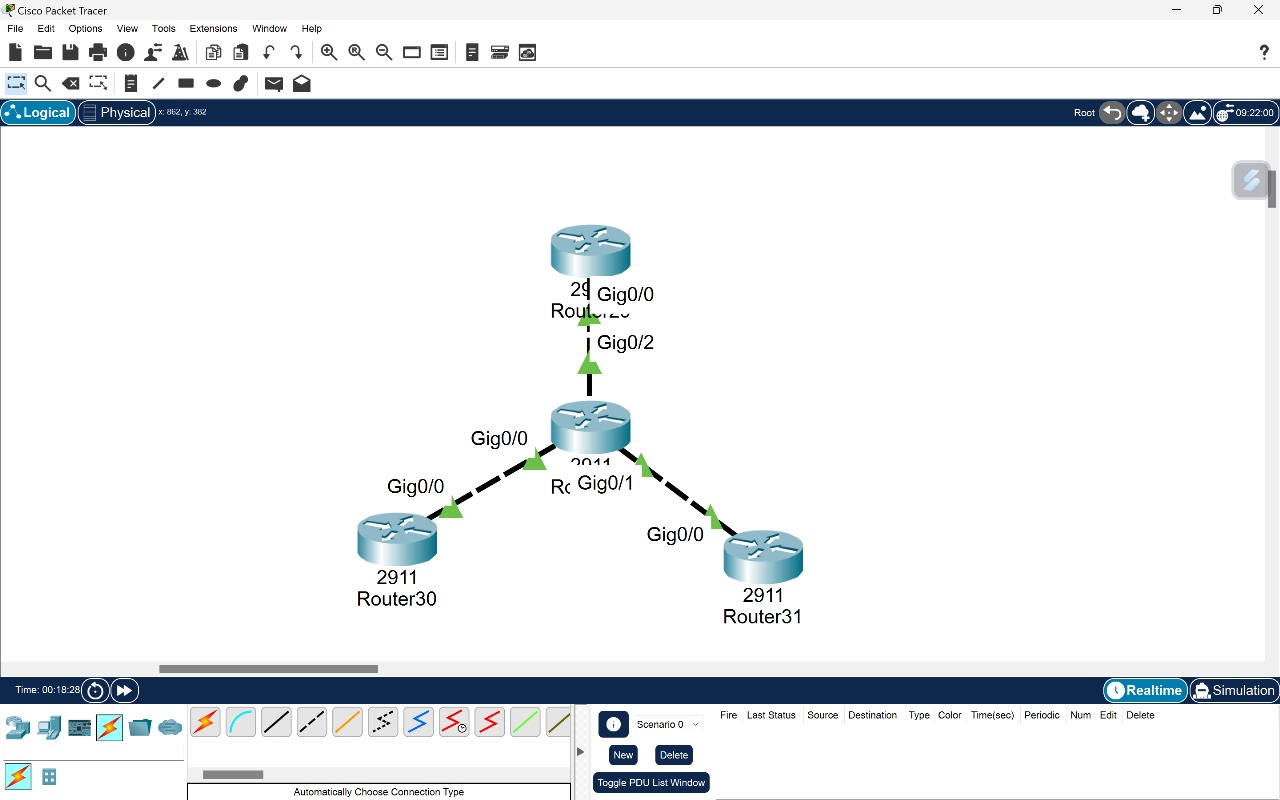
\includegraphics[width=0.6\textwidth]{img/point-multipoint.jpeg}
        \caption{Topologi 2: Point-to-Multipoint}
        \label{fig:topo2}
    \end{figure}
    \item Topologi 3: Wireless Bridging
    \begin{figure}[H]
        \centering
        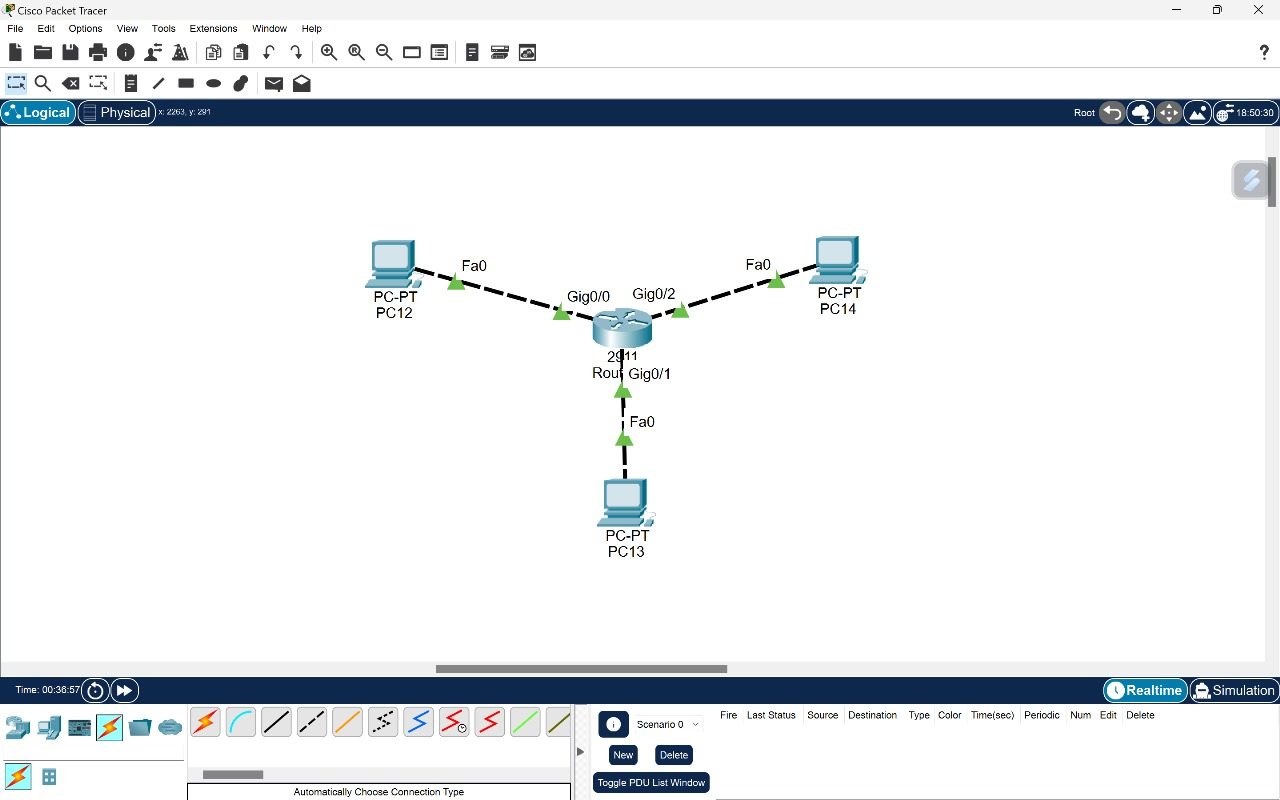
\includegraphics[width=0.6\textwidth]{img/wireless-bridging.jpeg}
        \caption{Topologi 3: Wireless Bridging}
        \label{fig:topo3}
    \end{figure}
\end{itemize}